\section{Hardware}

\subsection{Basisstation}

\newpage
\subsection{Sensor}

\begin{figure}[H] 
	\centerline{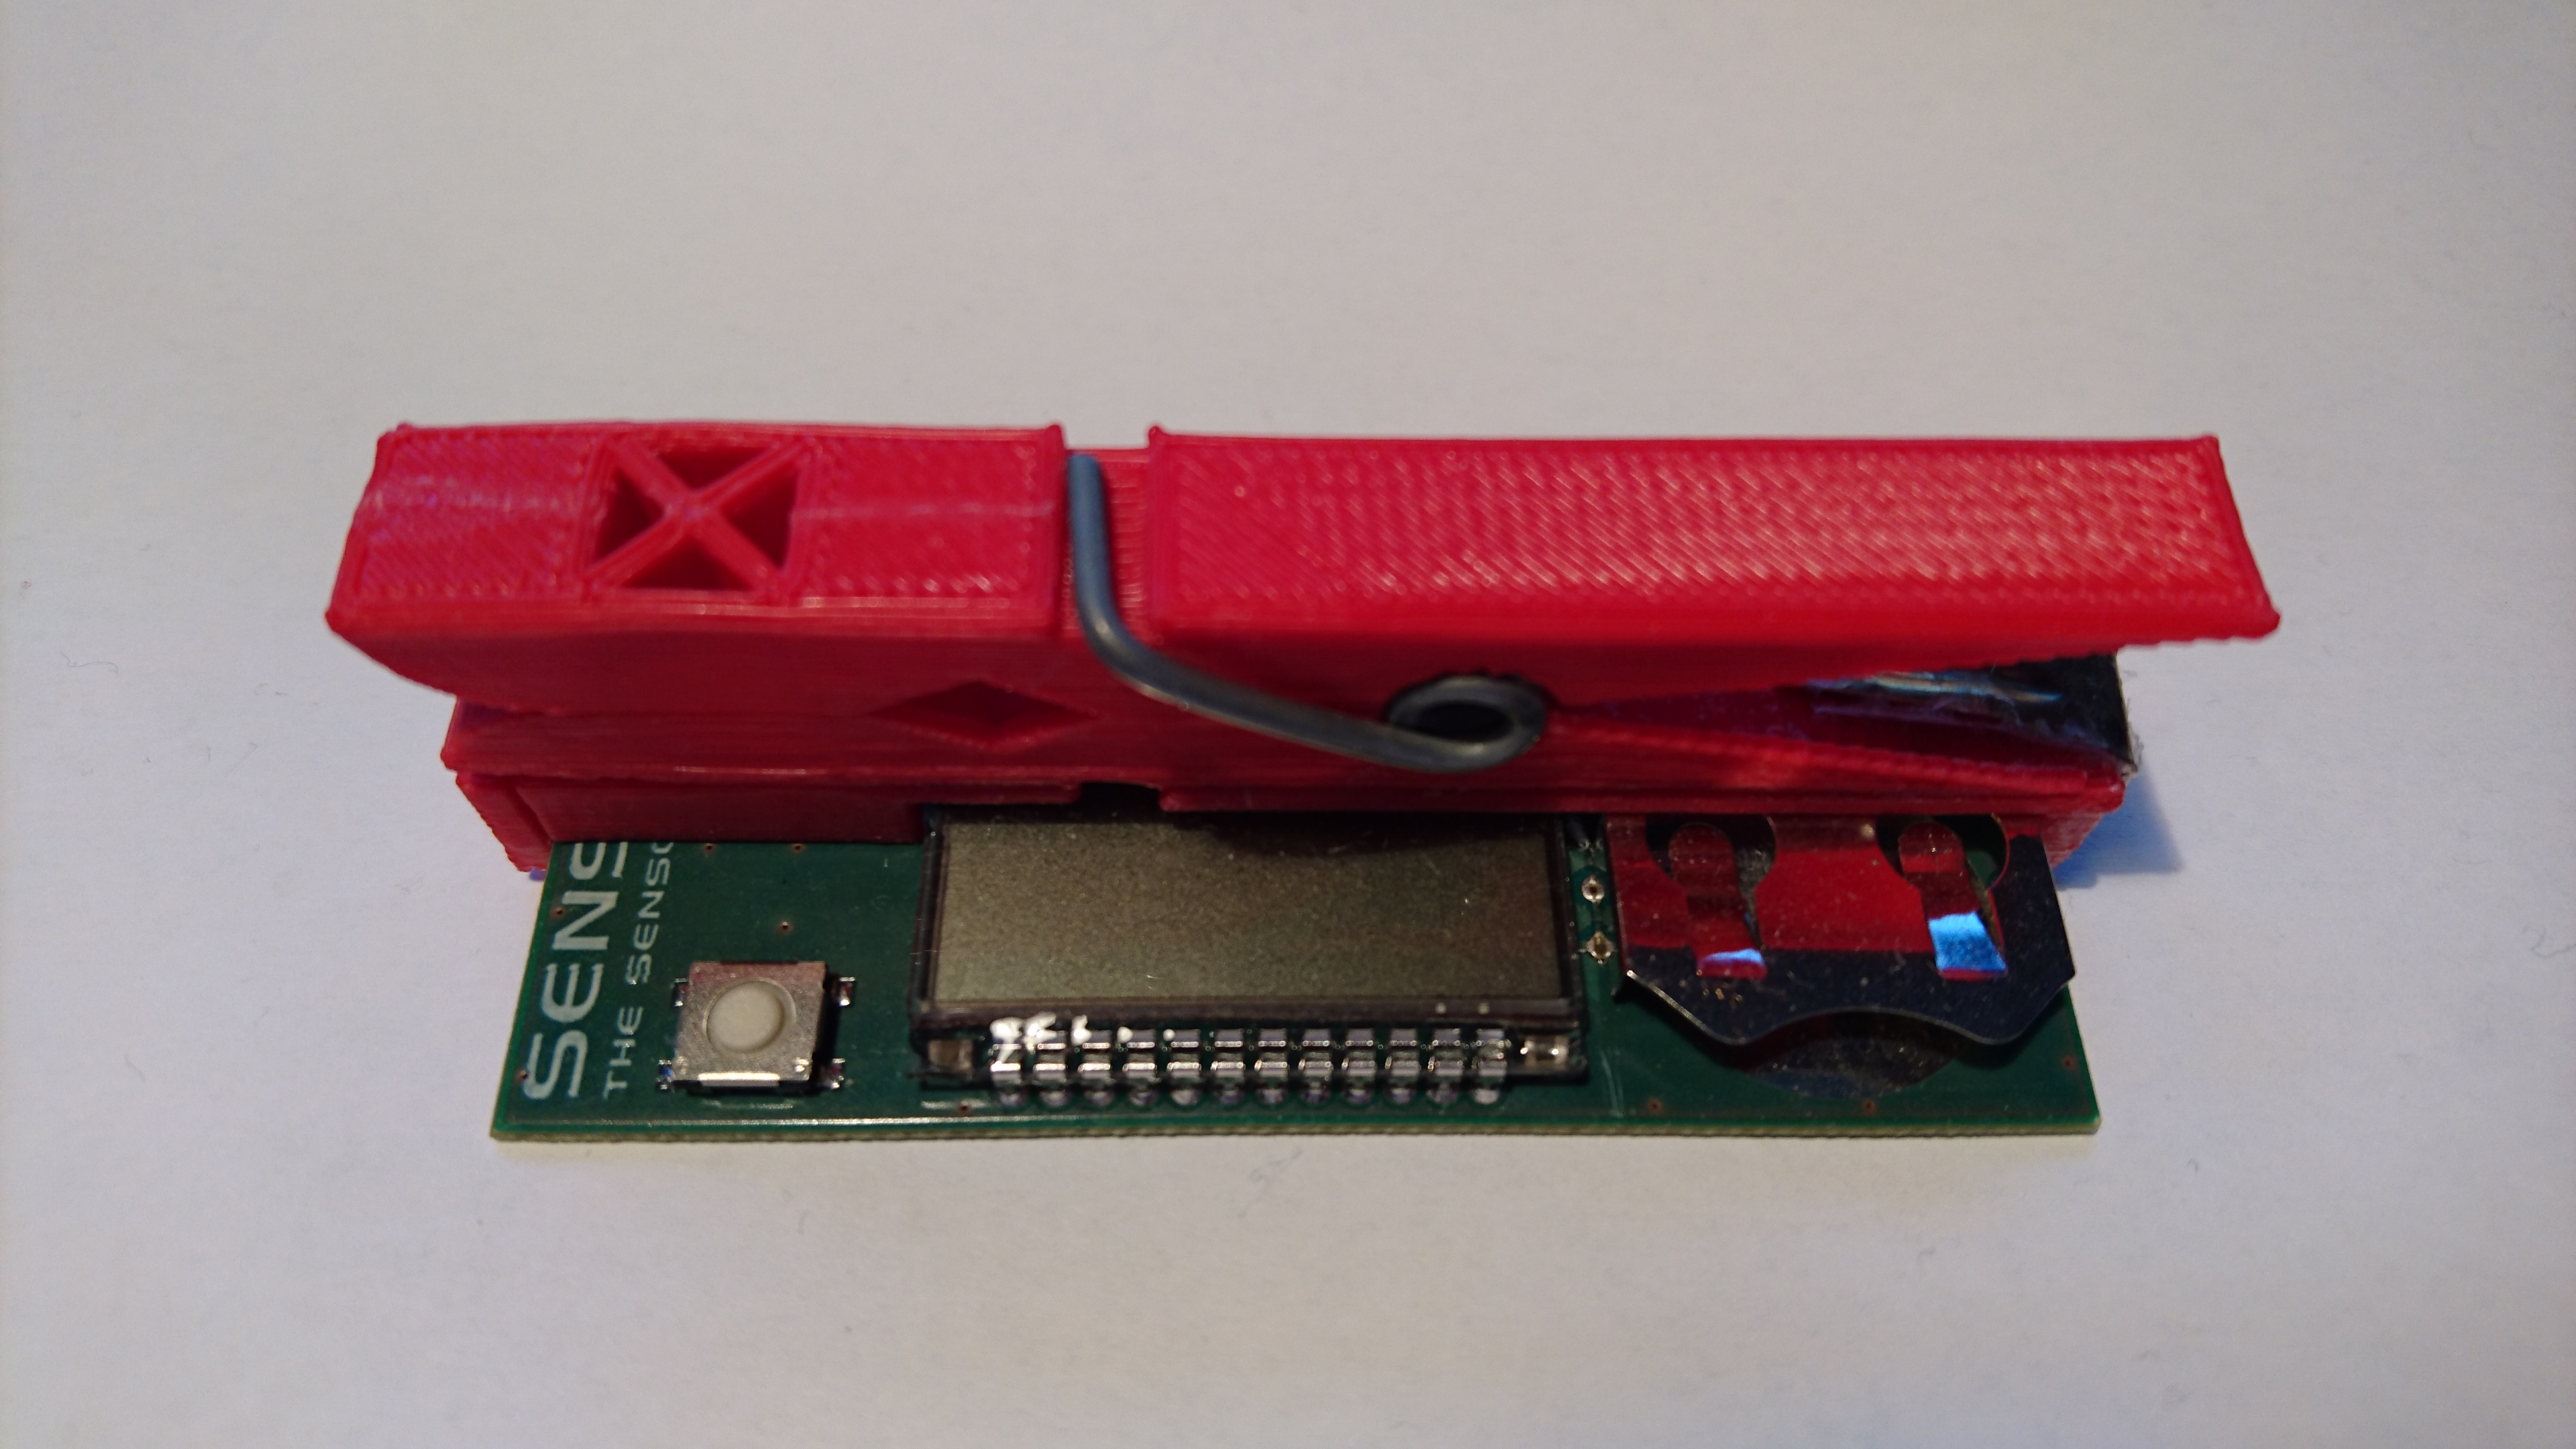
\includegraphics[width=1.0\textwidth]{sensor_seite_1}}
	\caption{Erste Seitenansicht}
	\label{sensor_seite_1}
\end{figure}

Der Sensor besteht aus einem Sensirion Smartgadget, sowie aus einer 3D gedruckten Klammer. Das Design der Klammer versucht 2 wesentliche Probleme zu lösen, nämlich einerseits die Befestigung des Smartgadgets, sowie andererseits die Erschaffung eines Zugangs des Feuchtigkeitssensors des Smartgadgets zur Wäsche, wodurch dieser die Feuchtigkeit der Wäsche messen kann.

\newpage
\begin{figure}[H] 
	\centerline{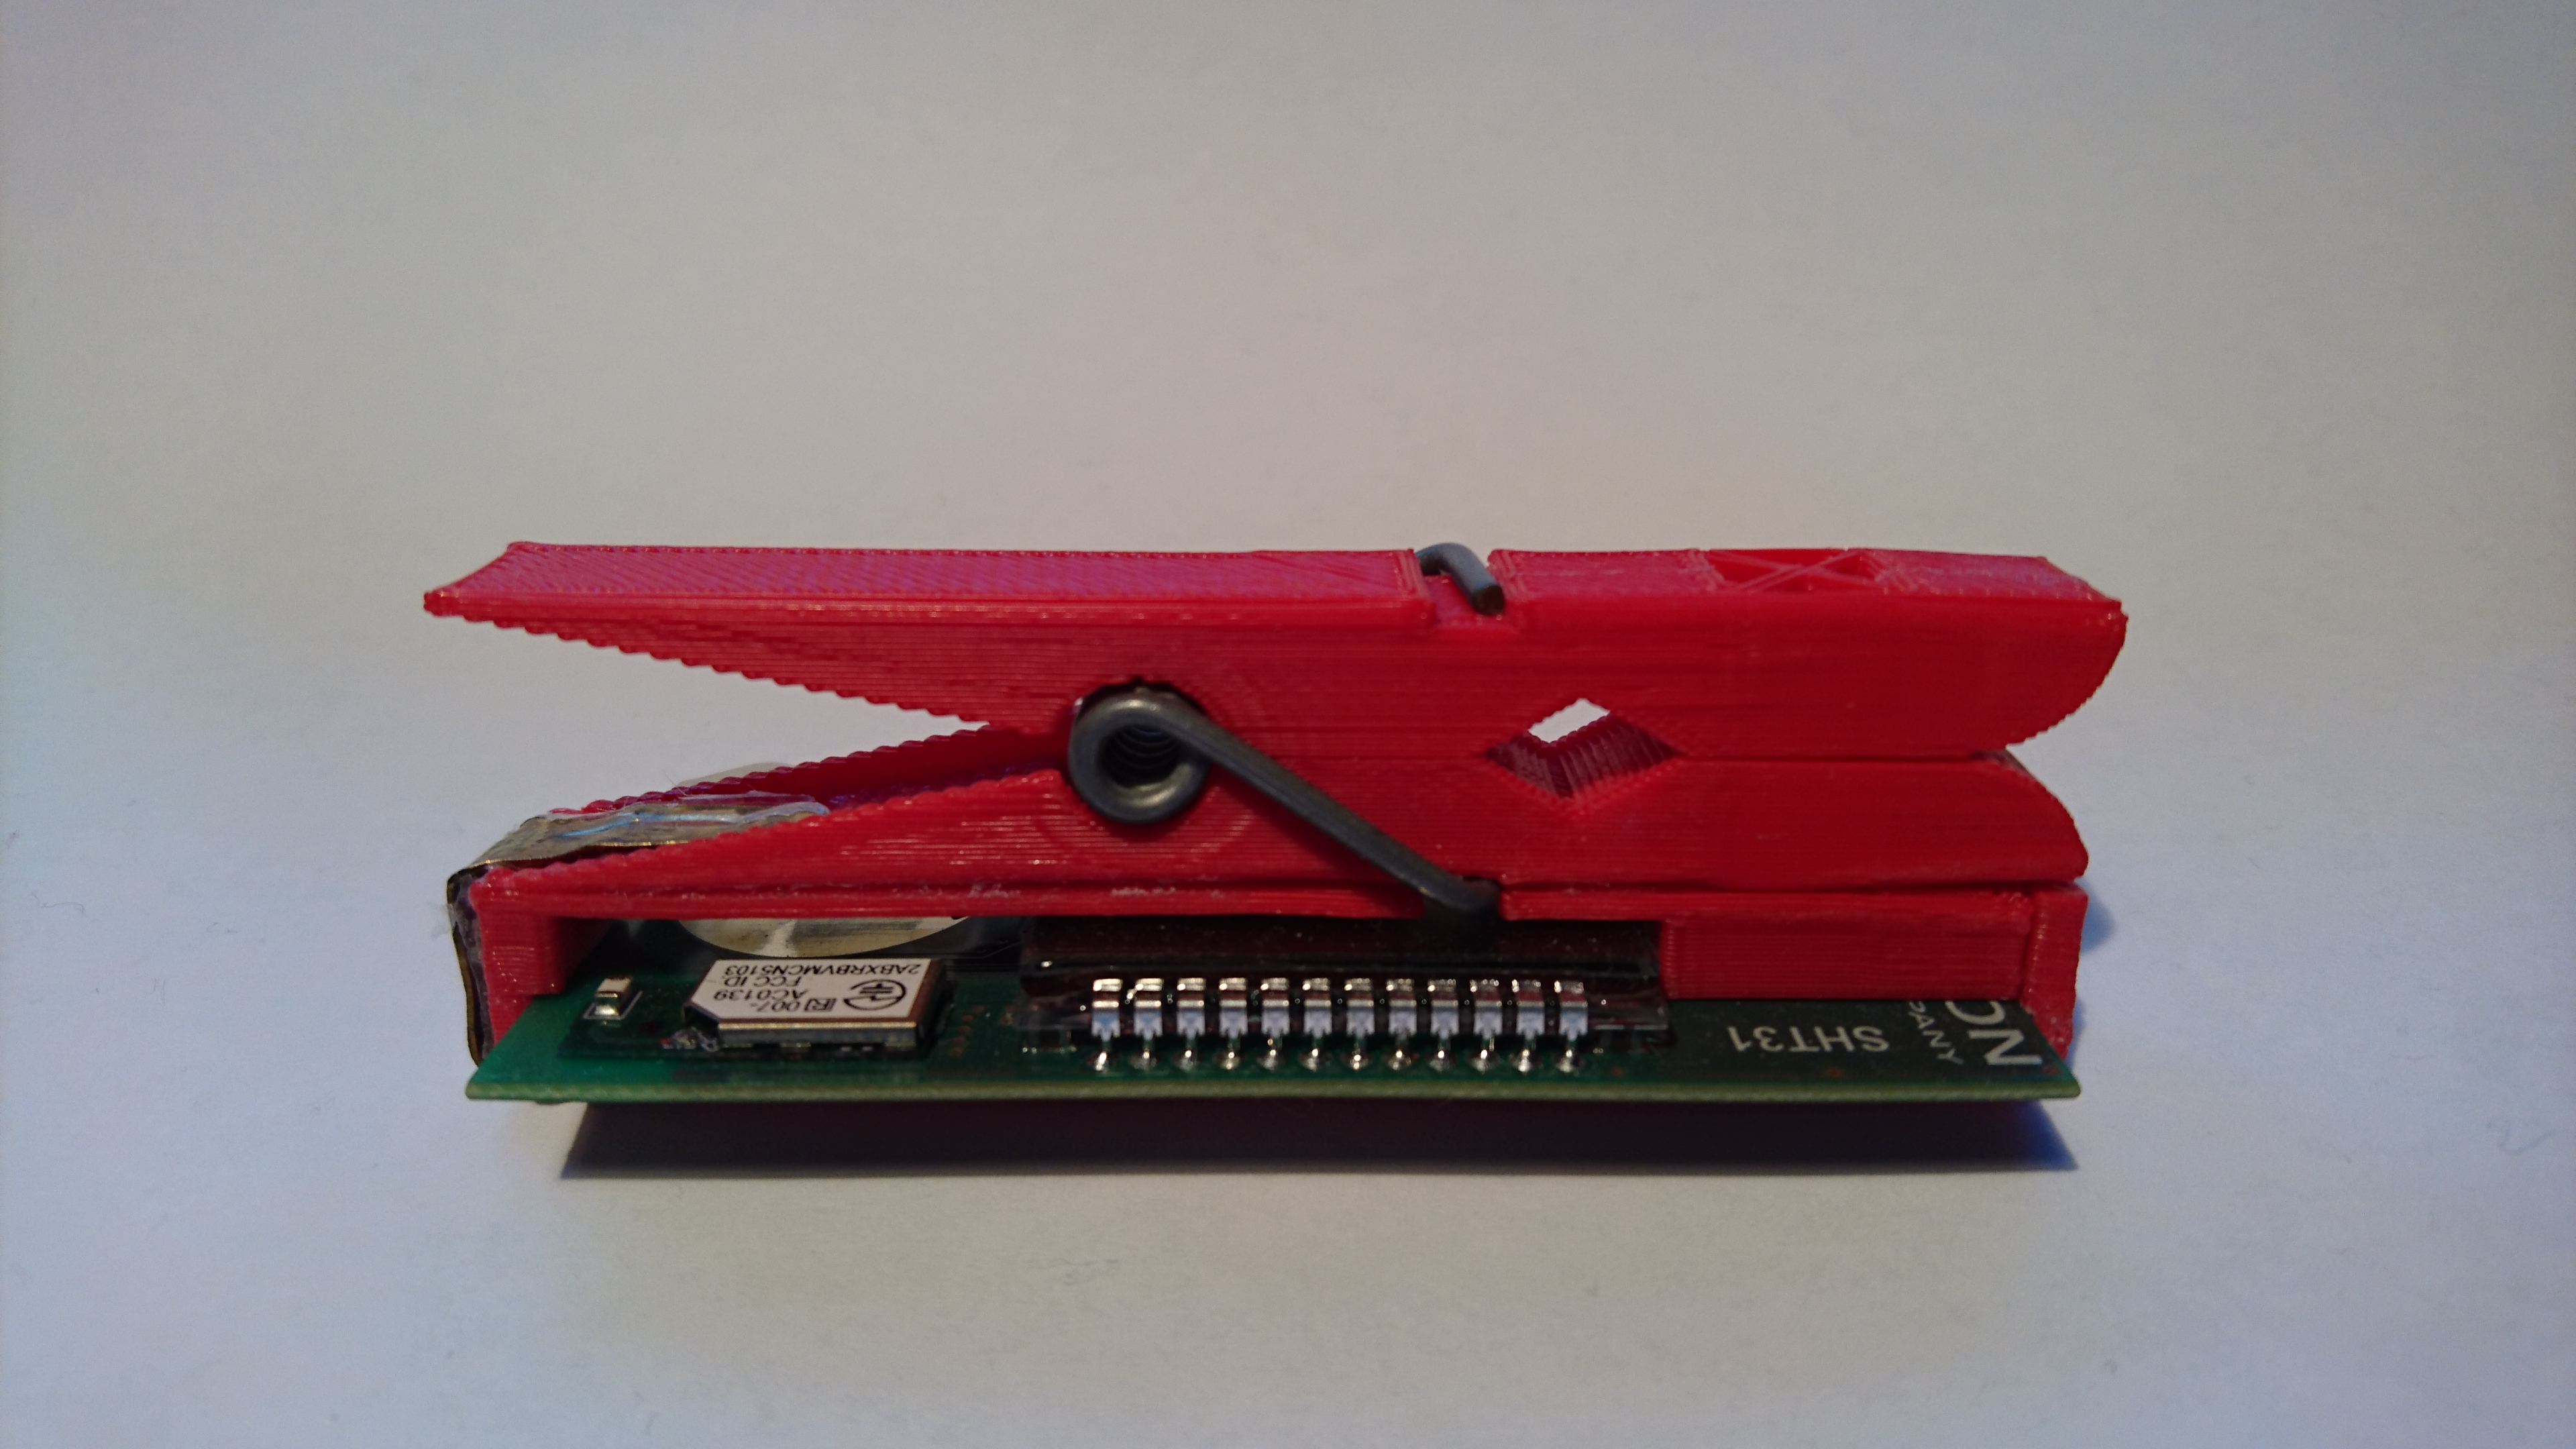
\includegraphics[width=0.8\textwidth]{sensor_seite_2}}
	\caption{Zweite Seitenansicht}
	\label{sensor_seite_2}
\end{figure}

\begin{figure}[H] 
	\centerline{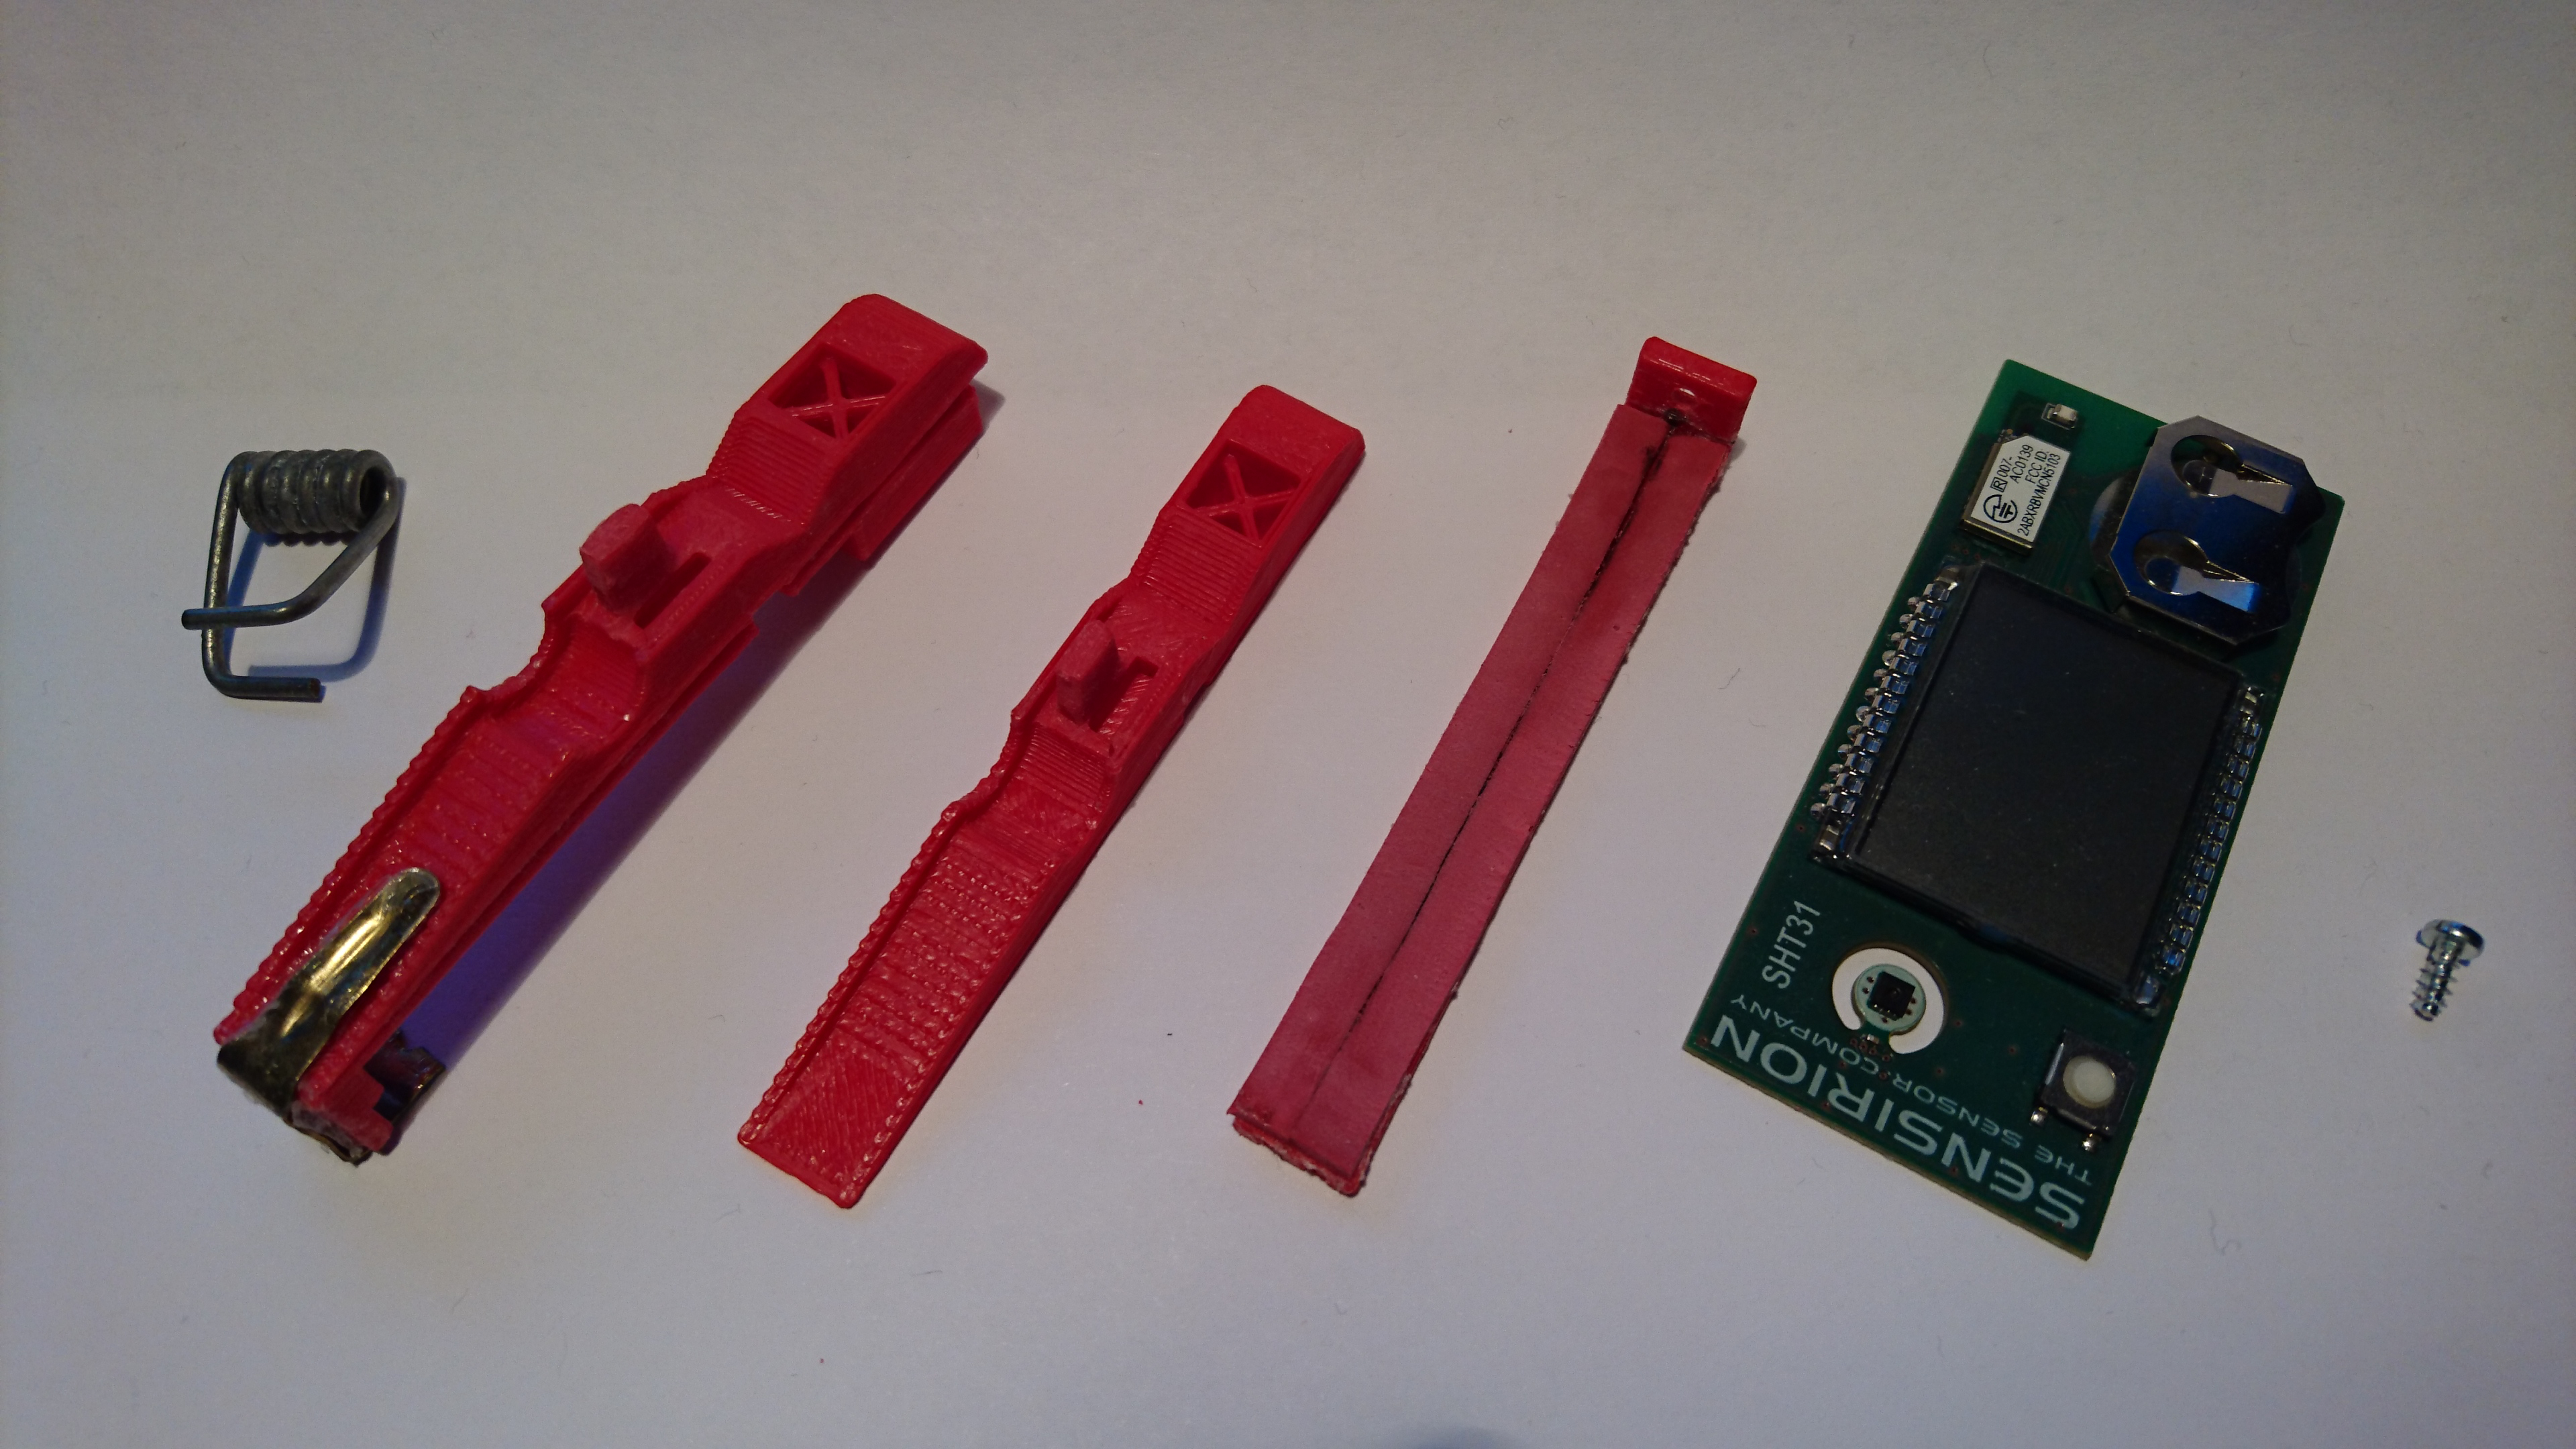
\includegraphics[width=0.8\textwidth]{sensor_teile}}
	\caption{Alle Einzelteile des Sensors. Hervorzuheben sind dabei die an der Schnalle (4. Teil von links) angebrachten Gummibänder, sowie die Öffnungen der oberen (2. Teil von links) und unteren (3. Teil von links) Klammerhälfte.}
	\label{sensor_teile}
\end{figure}

Um die Dimensionen der Klammer möglichst klein zu halten, wurde schon früh der Entschluss gefasst, dass sich das Smartgadget der langen Seite der Klammer entsprechend zu orientieren hat. Daraus folgt auch die letztliche Anordnung. Prinzipiell kann die Klammer in zwei Teile aufgefasst werden.

Das erste Teil ist dabei die Halterung, welche das Smartgadget über eine Schnalle fixiert. Die Schnalle besitzt zur weiteren Fixierung ein angebrachtes Gummiband, was durch Reibung ein Verschieben des Smartgadgets zumindest stark erschwert.

Das zweite Teil ist die eigentliche Klammer, welche konventionell aufgebaut ist und die Feder einer anderen Klammer enthält.

\begin{figure}[H] 
	\centerline{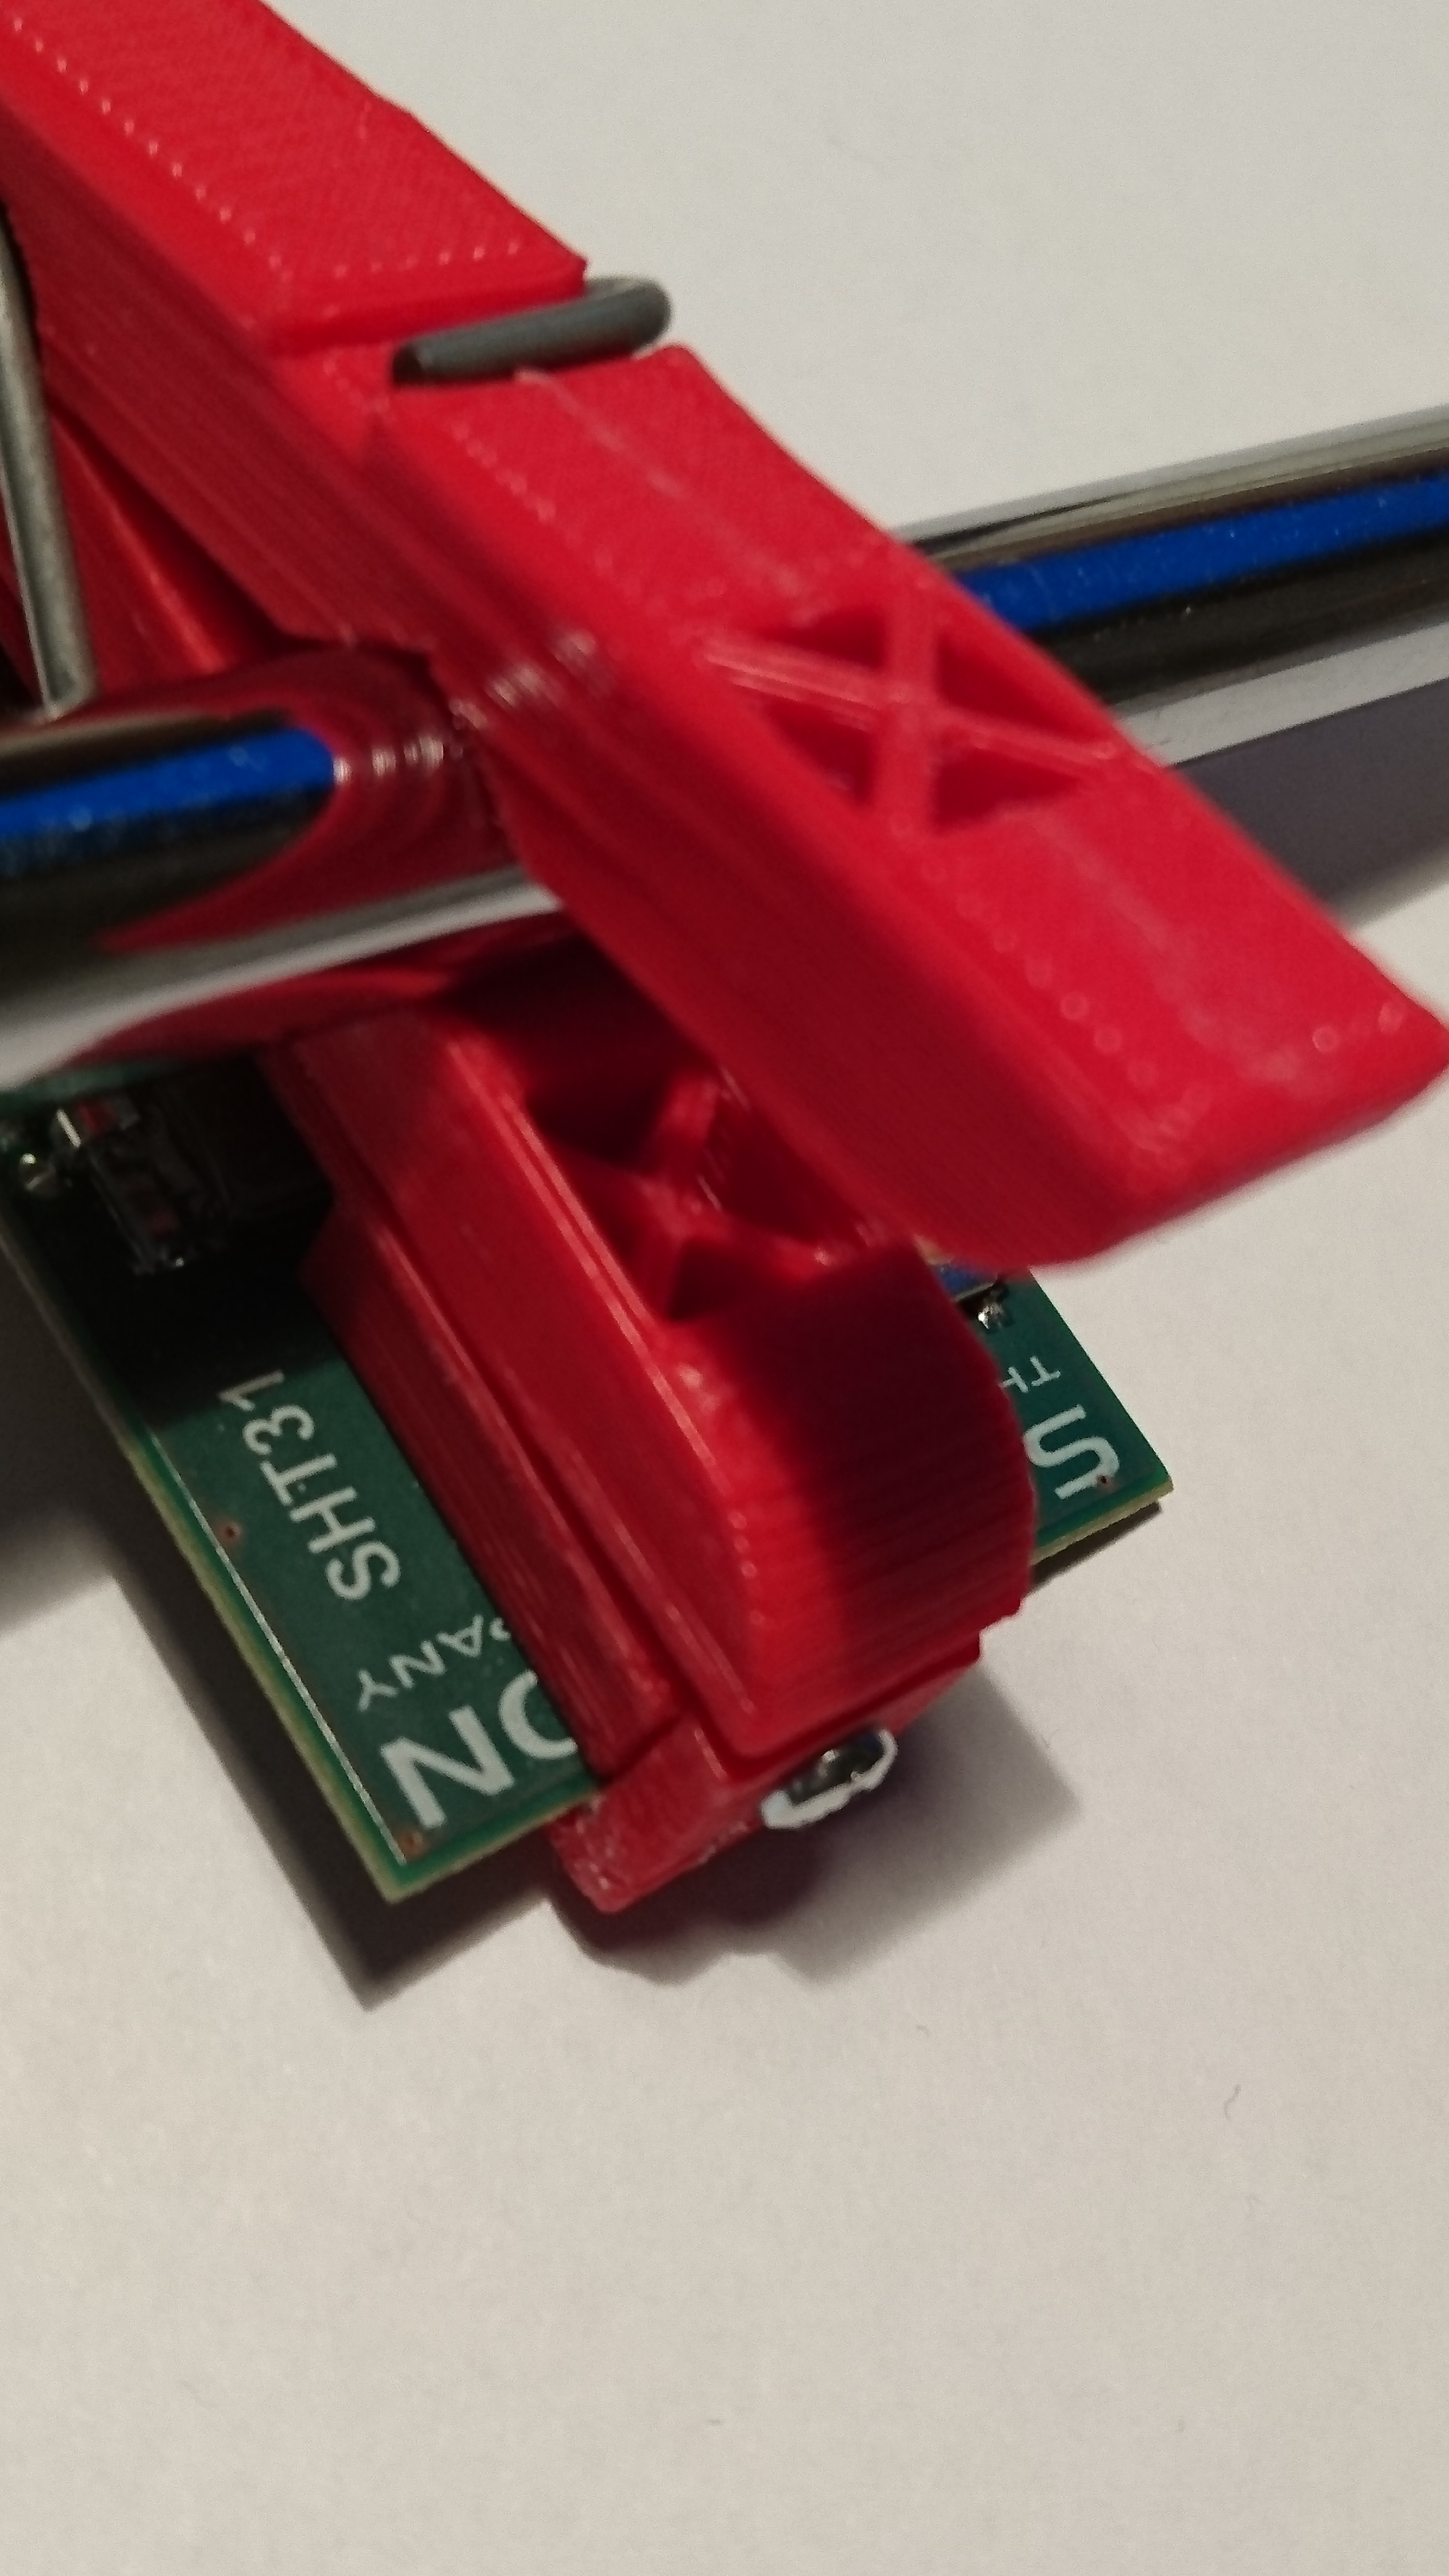
\includegraphics[width=0.5\textwidth]{sensor_oeffnung}}
	\caption{Die Öffnung des Feuchtigkeitssensors mit gegenüberliegender Öffnung für die Trocknung des relevanten Abschnitts der Wäsche}
	\label{sensor_oeffnung}
\end{figure}

Was den Zugang des Feuchtigkeitssensors zur Wäsche betrifft, wurde eine einfache Öffnung an der Vorderseite der Klammer geschaffen, in welcher sich der Feuchtigkeitssensor befindet.

Einerseits ist dadurch der gewollte Zugang geschaffen, jedoch ergibt sich auch das Problem, dass überhaupt kein Zugang zur Außenluft besteht und damit die Trocknung des relevanten Abschnitts der Wäsche stark eingeschränkt ist.

Um diesem Problem entgegenzuwirken, wurde eine zweite Öffnung geschaffen, welche der Ersten gegenüberliegt und das Wäschestück der Außenluft zugänglich macht. Auf diese Weise ist dann auch sichergestellt, dass der Feuchtigkeitssensor nicht direkt mit der Außenluft in Kontakt steht, sondern das Wäschestück als eine Art Membran den direkten Zugang blockiert.

\newpage
\subsection{Smartphone}
Für das Smartphone auf dem unsere Software läuft gibt es keine speziellen Hardware Anforderungen. Die App läuft auf allen Android Smartphones ab Android 4.0.3 und benötigt nur genügend Speicher und das Vorhandensein einer Netzwerkschnittstelle. Da unserer Applikation im Moment nur im gleichen Netz wie die Basisstation funktioniert sollte das entsprechende Telefon WLAN besitzen.